\documentclass{beamer}
\usepackage{mathtools}
\DeclarePairedDelimiter{\ceil}{\lceil}{\rceil}
\usepackage{algorithm}
\usepackage{algpseudocode}
\usepackage[english]{babel}
\usepackage[utf8]{inputenc}
\usetheme{Madrid}
\usecolortheme{dolphin}

\logo{\includegraphics[width=0.1\textwidth]{sdu_segl}}

\title{Interaktion og interaktionsdesign}
\author{Steven Gøhler}
\begin{document}
\begin{frame}
\titlepage
Redegør for den brugercenterede designproces.
\end{frame}

\begin{frame}
  \frametitle{Overview}
  \tableofcontents
\end{frame}

\section{Den brugercenterede designproces}
\begin{frame}
  \frametitle{Den brugercenterede designproces}
  \begin{columns}[T]
    \begin{column}{.5\textwidth}
	  \begin{itemize}
		\item Brugerkrav
		\item Træd ind i brugerens rolle
		\item Forudse brugerens forventninger
		\item Test på rigtige brugere
	  \end{itemize}
    \end{column}
    \begin{column}{.5\textwidth}
      \includegraphics[width=\textwidth]{UCD.pdf}
    \end{column}
  \end{columns}
\end{frame}


\section{Startpunkt}
\begin{frame}
  \frametitle{Startpunkt}
  \begin{columns}[T]
    \begin{column}{0.5\textwidth}
      \begin{itemize}
	    \item Brugerkrav, konceptuel model
	    \item Sæt dig ind i rollen
	    \item Undersøg muligheder
	    \item Alternativer
      \end{itemize}  
    \end{column}
    \begin{column}{.5\textwidth}
      
\includegraphics[width=\textwidth]{research.jpg}
    \end{column}
  \end{columns}
\end{frame}


\section{Designet}
\begin{frame}
  \frametitle{Designet}
  \begin{columns}[T]
    \begin{column}{0.5\textwidth}
      \begin{itemize}
	    \item Ud fra research
	    \item Hvilke forventninger?
	    \item Førstehåndsindtryk
	    \item Prototyper
      \end{itemize}  
    \end{column}
    \begin{column}{.5\textwidth}
      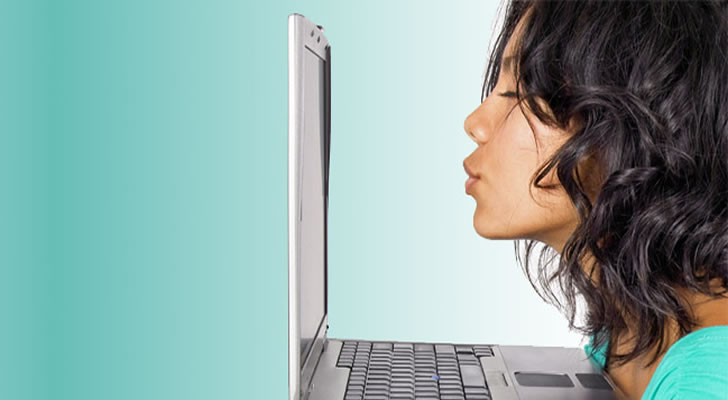
\includegraphics[width=\textwidth]{loveit.jpg}
    \end{column}
  \end{columns}
\end{frame}


\section{Tilpasninger}
\begin{frame}
\frametitle{Tilpasninger}
  \begin{columns}[T]
    \begin{column}{.6\textwidth}
	  \begin{itemize}
		\item Prototype testning af brugerne
		\item Bedste fra hver
		\item Hvad skal ændres?
		\item Tilbage til tegnebrættet
		\item Endelige produkt
	  \end{itemize}
    \end{column}
    \begin{column}{.4\textwidth}
      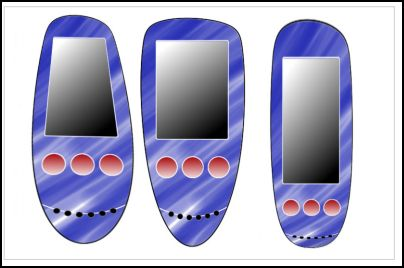
\includegraphics[width=\textwidth]{alt.jpg}
    \end{column}
  \end{columns}
\end{frame}


\end{document}